\documentclass[11pt, letterpaper]{article}
\usepackage{graphicx}
\title{Lab T report}
\begin{document}
\maketitle
\section{Administrative}

Team names: Graham Benevelli Jake Wilke\\
Team uteids: grambo jlw3599\\
Slip days previously used: 0\\
Slip days used this project: 0\\
Slip days remaining:5\\

\section{Part 1: Basic synchronization}

{\em Stats keeps track of the bytes already being sent in an array. When a call to update is made the number of bytes passed is added to the array at the threads flowId. As this goes on max_id updates so we don't print out too much information. When toString is called the data in the byte_array is formatted into the passed buffer string. Then the byte_array is reset to zero so that it can keep track of the next batch of data.}

\subsection{Evaluation}

\centerline{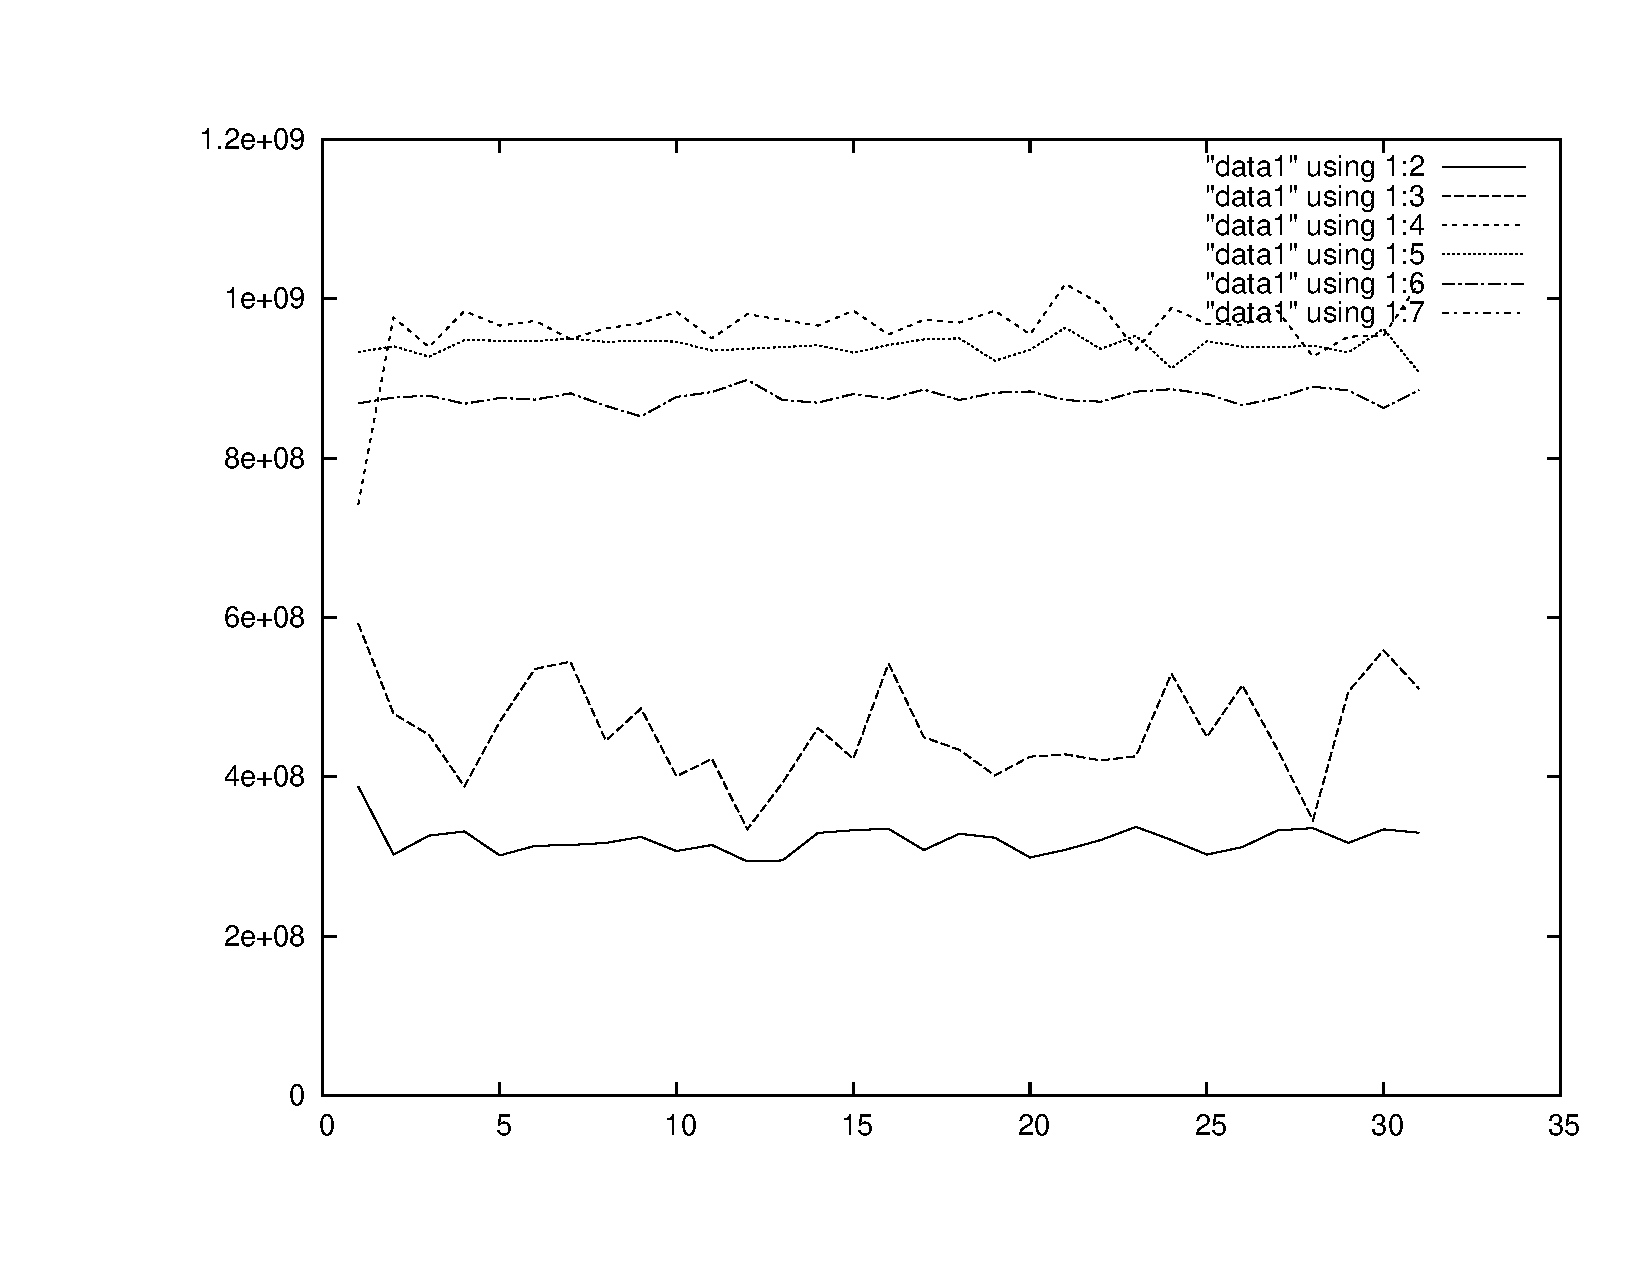
\includegraphics[width=3in]{plot1}}

{\em It shows that data is being processed at a very high rate, mostly because no bound was put on the data. So more then 2-4 million bytes is transmitted by each thread, giving around a total of 1.2 billion bytes a second.}


\centerline{
\includegraphics[width=3in]{plot1b}}

{\em The graph shows that bytes transmit at almost exactly the same but with a cut off on the total. This test transmitted data until about 15 second then dies and no longer has data to transmit. At the end you see a spike in a few of the treads lines. This is because other threads finish their work early giving the ones left more time with the processor. That way they can transmit a higher rate for a short period of time. What we found was odd because plot1b seems to run at a slower overall rate than plot1. }



\section{Part 2: MaxNWScheduler}

{\em We have some synchronization variables to ensure that only one thread is trasmitting data at once and under the correct transfer rate. This is accomplished by used deadlines, calcuated by the alarm thread, that will sleep until the deadline is met. We keep track of these through three integers. We have two methods, waitMyTurn() and signalNextDeadline(), that do the brunt of the work. waitMyTurn() will first wait to see if another thread is sending any data. When current running thread is done waiting, then the it will send a message that a new deadline needs to calculated. The alarm thread will consistently call signalNextDeadline(). When this method is called, it will check to see if any new data needs to be transmitted. If so, then it calculates the next deadline and broadcasts to all other waiting threads.}

{\em We can sendAndRecv numerous times to view the resulting data. We then spot checked the result to see what and if there were any mistakes. }

{\em We came up with two ways of approaching the signalNextDeadline to make sure that there is no rounding error. One used the current time to set the next deadline, this one is safer and simulates a working system better. So keeping at the current time it would sometimes go over the rate. The other way makes sure to round up when over the new deadline is calculated. }


\subsection{Evaluation}

\centerline{
\includegraphics[width=3in]{plot2}}

{\em The graph shows four threads all running at about the same speed but at a varying rate. Overall the total amount of bytes transmitted stays below a million bytes a second. }


\centerline{
\includegraphics[width=3in]{plot2b}}

{\em This graph shows the same thing. The four threads run at the same varying rate with an overall rate below a million. But since this graph has a bound the transfer rate drops off at about 27 seconds. }






\section{Part 2: MaxNWScheduler}

{\em At most 1/2 page -- Discuss high level design, any issues/known
  bugs for part 2}

{\em Discuss your testing strategy -- what tests did you run, what were the
results?  (Feel free to include graphs in your turnin.) You should
provide instructions for the TA to run your tests, but you should also
make sure that the results of your runs (graphs, data files, etc.) are
in files that will not be overwritten if the TA tries to reproduce
your results.}

{\em Anything the TA needs to know about when grading part 2? Known bugs?
Interesting design points?}


\subsection{Evaluation}

\centerline{
\includegraphics[width=3in]{plot3}}

{\em Explain graph; identify/explain any
  interesting/unexpected/important features}

\centerline{
\includegraphics[width=3in]{plot3b}}

{\em Explain graph; identify/explain any
  interesting/unexpected/important features}

{\em Insert any other graphs or test results along with
  discussion/explanation here}





\end{document}


